% !TeX root = ../FinalRepordCS.tex

\chapter{Implementation and Preliminary Performance Analysis}

\section{Implementation}
In this section, the main focus is on implementing the functions of LoRa nodes Alice and Bob through the Arduino programmable MCU board and IDE mentioned earlier, in conjunction with the LoRa frequency modulation chip and the algorithms mentioned above.

\section{Deep-in-Building and Outdoor Test}
In this section, I conducted a test to generate LoRa physical layer keys in a practical application scenario. The test provided positive results, demonstrating the practical application of LoRa in real-world scenarios. Moreover, the findings are of significant reference value for the future utilization of the LoRa protocol in environmental monitoring.

\subsection{RSSI Pairs Generation}

\begin{figure}
  \centering
  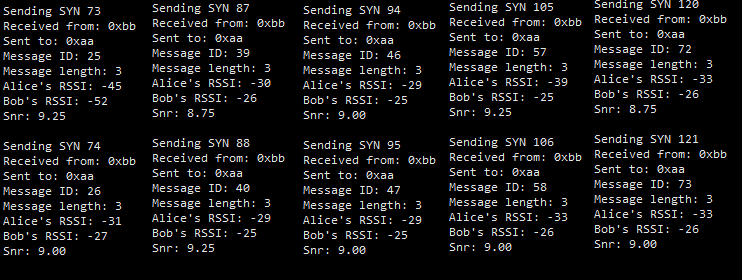
\includegraphics[width=0.9\linewidth]{fig5-1.png}
  \caption{Sampling in LoRa Node}
  \label{fig:5-1}
\end{figure}

\subsection{Key Generation}
I implemented a Python Program constitutes a crucial section of the thesis, focusing on LoRa physical layer key generation. Beginning with the processing of Received Signal Strength Indication (RSSI) data for both Alice and Bob, the code subsequently employs linear interpolation and Savitzky-Golay filtering to enhance the quality of the data.

Following these preprocessing steps, the script employs M-ary quantization on the smoothed RSSI values, utilizing a specified number of bits per sample and an alpha parameter. The homotopy method for error correction is then implemented, where a matrix A and vector y undergo iterative updates to correct errors in the data.

The key generation process involves the random generation of a matrix A, the computation of vectors y1 and y2 based on the quantized data from Alice and Bob, and the application of error correction through the homotopy method. The final step involves XORing the original bits with the corrected bits to derive the cryptographic key.

The code also incorporates visualizations using Matplotlib to illustrate the impact of linear interpolation and Savitzky-Golay filtering on the original RSSI values. Additionally, the thesis section concludes with the presentation of crucial output information, including filtered RSSI arrays for Alice and Bob, and the original and corrected keys for Alice. It is imperative to ensure the existence and proper format of the input file containing RSSI values (sampling1.txt) before executing the code.
\begin{figure}
  \centering
  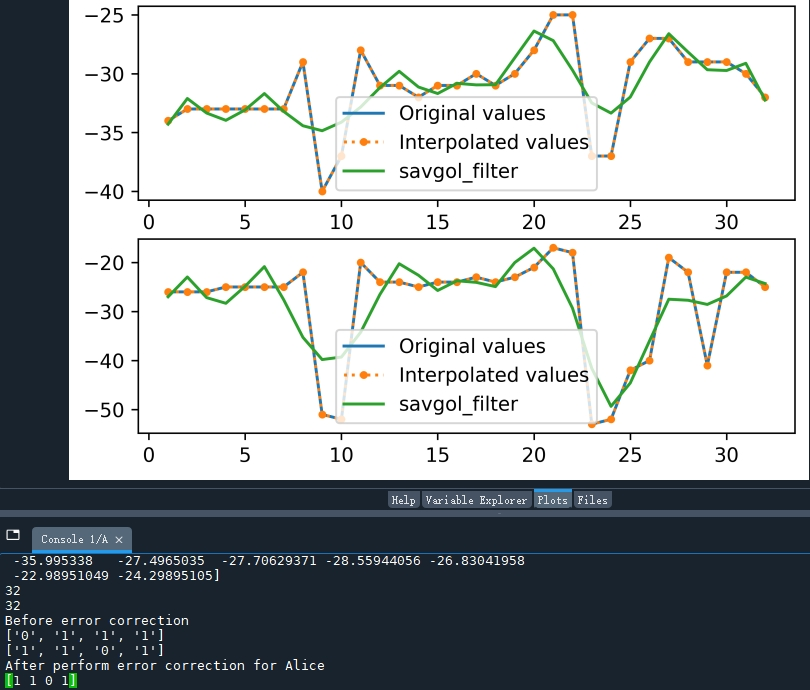
\includegraphics[width=0.9\linewidth]{fig5-2.png}
  \caption{Result of Perform Key Generation}
  \label{fig:5-2}
\end{figure}

\subsection{Data Encrypt and Decrypt}

\section{Performance Analysis}
In this section, performance tests on password generation were implemented based on references, exploring the impact of different parameters. Additionally, the results were visualized for better comprehension of the test data.
